
\begin{figure*}[!t]
\centering
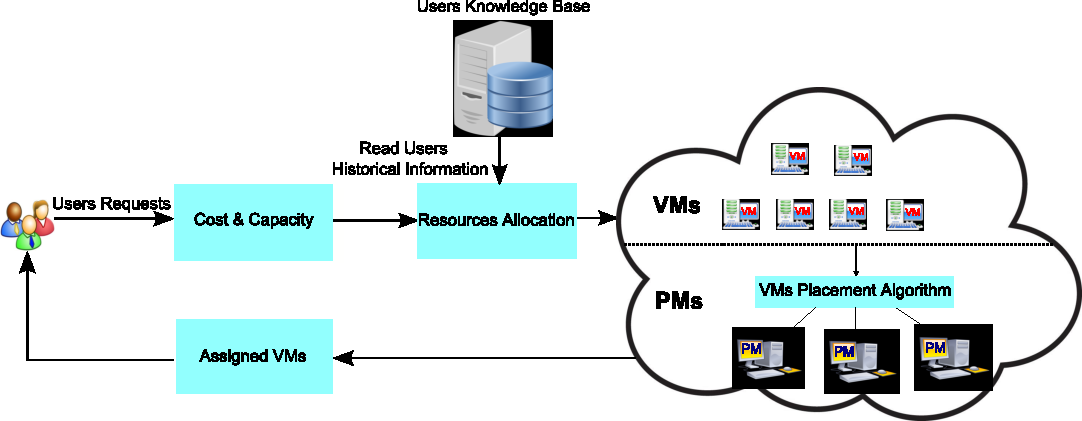
\includegraphics[width=7in]{pic/frame.pdf}
\caption{Work flow diagram showing Churn Aware Cloud Computing Framework}
\label{frame}
\end{figure*}

Our goal in this paper is to address customer churn problem in cloud computing businesses by improving the customer satisfaction while maximizing the total profit. Our problem scenario includes customers with certain SLAs, level of satisfaction and finding the best VMs placement strategy in cloud environment. Therefore, the related work section is subdivided into three parts, the dynamics of customer churn, retention and profitability, customer churn identification, and resource allocation and placement for profit maximization/cost minimization in cloud. 
\subsection{Customer Churn, Retention and Profitability}
%This is an example of a subsection title that needs to be changed to something we will be possibly using


A theoretical framework on customer retention and maximization of profit is presented in~\cite{lemmens2013managing}. Proposed work describes a relation between individual customer value and retention action, which is a popular and effective way to keep the customers and reduce the churn rate. Data mining models to predict customer churn in B2B along with profitability metric to maximize the profit of a retention campaign is proposed in~\cite{TamaddoniJahromi20141258}. This study concludes that model driven approach to churn management outperforms managerial heuristics. Several  important  considerations, including  the  value  of  cohorts,  types  of 
future revenue, and how to model retention and lifetime value for cloud business are explored in~\cite{cloudchurn2012}. This study shows how  churn  can  completely  undermine  a  seemingly  healthy cloud business. 


\subsection{Churn Identification}

The cloud providers need to predict and calculate the churn rate based on historical customer data. There have been several work on machine learning framework for identification and prediction of churners in a business. The framework in ~\cite{fasanghari2011customer} relies on a local linear model tree to identify and predict future churners in an iranian telecommunication companies. A neural network approach is proposed in~\cite{hadden2008customer}. In \cite{buckinx2007predicting}, a multiple linear regression model is developed to predict a customer’s behavioral loyalty by using the transactional database. 
Another machine learning framework to address churn problem in telecommunication is proposed in~\cite{obiedat2013customer}       .  The technique proposed in this work uses a hybrid genetic programming method is used where first, K-means  clustering  is used  to  filter outliers and non  representative  customer  behaviors  from training data, then Genetic  Programming  is  applied  to 
build classification trees to distinguish churners from  non  churners. It is to be noted that our work uses a Bayesian classifier approach which is computationally efficient.
 
\subsection{Economics in Resource Allocation and Placement}
This subsection describes some notable work on economics in resource allocation and placement. Cloud computing related work on improvement in customer satisfaction is presented in~\cite{chen2011tradeoffs} where customers’ satisfaction is abstracted and quantified in an auction framework.  Workload model and the failure correlations to redirect requests to appropriate cloud providers is considered in~\cite{javadi2012hybrid}, furthermore, evaluation of performance and monetary cost of the proposed policies is performed. Resource allocation strategy in cloud computing clusters and physical machines is proposed to maximize the overall profit in~\cite{goudarzi2011maximizing}. A combinatorial auction-based resource allocation protocol is proposed in~\cite{das2005combinatorial} and its economic efficiency and its effect on the system performance is computed. Deadline aware workflow scheduling algorithim is proposed in~\cite{abrishami2013deadline}. Algorithms to optimize work-flow scheduling and to reduce total resource provisioning cost are proposed in~\cite{chaisiri2010robust}. The extension of the work that includes various computation resources is found in~\cite{chaisiri2012optimization}. Research on billing strategies that involve various cloud computing resources ins presented in~\cite{li2012research}.

Our resource allocation and placement strategy includes both, interference and operation overhead~\cite{lin2012interference, li2013performance} of virtual machines. Interference and operation overheads affect practical VM placement on physical machines, therefore, it affects the cost.
%In the paper \cite{lin2012interference}, they looked into IAVMP problem and offer a heuristic algorithm to solve it. Li et al. \cite{li2013energy} focused on online VMs placement to minimize the total consumption and to decrease the number of fragments. Finally, when we considered response time, a paper \cite{li2014task} mentioned an algorithm of scheduling, and researchers divided the task into several parts and allocate them.



